\documentclass[11pt]{article}

\usepackage[T1]{fontenc}
\usepackage[utf8]{inputenc}
\usepackage{lmodern}
\usepackage{microtype}
\usepackage[letterpaper,top=1.0in,bottom=1.0in,left=1.1in,right=1.1in]{geometry}
\usepackage{amsmath,amssymb,amsthm,mathtools}
\usepackage{booktabs}
\usepackage{array}
\usepackage{enumitem}
\usepackage{xcolor}
\usepackage[numbers,sort&compress]{natbib}
\usepackage{tikz}
\usetikzlibrary{arrows.meta,positioning,calc,shapes.geometric,backgrounds,fit}
\usepackage{pgfplots}
\pgfplotsset{compat=1.18}
\PassOptionsToPackage{hyphens}{url}
\usepackage[colorlinks=true,linkcolor=MidnightBlue,citecolor=TealBlue,urlcolor=MidnightBlue,pdftitle={Beyond Unions and Concatenations: Lawvere-Amari Generative Skill Manifolds for Compositional Agentic Systems},pdfauthor={SkillCompose Research}]{hyperref}
\usepackage[nameinlink,noabbrev]{cleveref}

% Okabe-Ito colorblind-safe palette
\definecolor{MidnightBlue}{HTML}{004488}
\definecolor{TealBlue}{HTML}{0072B2}
\definecolor{Vermilion}{HTML}{D55E00}
\definecolor{BluishGreen}{HTML}{009E73}
\definecolor{AmberGold}{HTML}{E69F00}
\definecolor{SlateGray}{HTML}{4A5568}
\definecolor{SoftBg}{HTML}{F7FAFC}

% Theorem environments
\theoremstyle{definition}
\newtheorem{definition}{Definition}
\theoremstyle{plain}
\newtheorem{theorem}{Theorem}
\newtheorem{proposition}{Proposition}
\newtheorem{lemma}{Lemma}
\newtheorem{corollary}{Corollary}

% Mathematical macros
\newcommand{\Xcal}{\mathcal{X}}
\newcommand{\Ycal}{\mathcal{Y}}
\newcommand{\Ucal}{\mathcal{U}}
\newcommand{\Dcal}{\mathcal{D}}
\newcommand{\Fcal}{\mathcal{F}}
\newcommand{\Mcal}{\mathcal{M}}
\newcommand{\Tcal}{\mathcal{T}}
\newcommand{\Ncal}{\mathcal{N}}
\newcommand{\Lcal}{\mathcal{L}}
\newcommand{\Pcal}{\mathcal{P}}
\newcommand{\Gfrak}{\mathfrak{G}}
\newcommand{\Phicore}{\Phi_{\mathrm{core}}}
\newcommand{\KL}{D_{\mathrm{KL}}}
\newcommand{\Ebb}{\mathbb{E}}
\newcommand{\Rbb}{\mathbb{R}}
\newcommand{\Cov}{\mathrm{Cov}}

\setlength{\parskip}{3pt}
\setlength{\parindent}{15pt}
\emergencystretch=1.2em

\title{%
  \vspace{-1.2em}
  \rule{0.94\textwidth}{1.5pt}\\[0.55em]
  {\LARGE\bfseries Beyond Unions and Concatenations: Lawvere--Amari Generative Skill Manifolds for Compositional Agentic Systems}\\[0.45em]
  \rule{0.94\textwidth}{0.7pt}
}

\author{%
  \textbf{SkillCompose Research}\\[0.25em]
  {\small Open-Source Reference Implementation \& Benchmark:}\\[0.1em]
  {\small \url{https://github.com/thehalleyyoung/skillcompose}}
}
\date{}

\begin{document}
\maketitle

\begin{abstract}
\noindent
Modular skill libraries equip language-model agents with reusable domain procedures, yet composing multiple skills for tasks that span several operational constraints remains brittle. Naive prompt concatenation takes the logical conjunction of all member specifications, which collapses onto an empty admissible output set whenever standalone skills prescribe conflicting local defaults, and leaves the agent unguarded against off-domain requests. Conversely, discrete skill-union routing selects a single member skill per query, confining generation to the union of individual skill supports and failing cross-artifact consistency on multi-stage tasks. We address both failure modes by formulating a skill not as a static text prompt, but as a guarded conditional generative transducer mapping each input to a constrained fiber of structured multi-view outputs. From a finite set of landmark skills, we construct a \emph{Lawvere--Amari Generative Skill Manifold} ($\Gfrak_{\Mcal}$) that unifies two dual structures: (i) an exponential-family statistical submanifold equipped with the conditional Fisher--Rao metric, whose $e$-geodesics synthesize multiplicative product-of-experts intersections across skill fibers, and (ii) a fibered logical specification combining a Galois-closed conormal core of universal safety invariants with Plotkin--Reynolds anti-unification of conflicting regime defaults and \v{C}ech sheaf gluing across coupled output views. To select landmark skills from noisy repositories, we prove that combining noisy-OR role coverage with the D-optimal Fisher log-determinant volume yields a monotone submodular objective with constant-factor optimality certificates, while a read-only post-dominator verification gate breaks the Data Processing Inequality of pure-prompt chains. Across seven concrete task families evaluated with one isolated agent call per task and regime, $\Gfrak_{\Mcal}$ achieves a $98.71/100$ mean double-blind judge score, a $100.0\%$ ($7/7$) exogenous verification pass rate, and $7/7$ blind first-place wins over prompt concatenation ($87.27/100$, $0/7$ wins) and skill-union routing ($53.66/100$, $0/7$ wins).
\end{abstract}

% ============================================================================
\section{Introduction}
\label{sec:intro}

Language-model agents increasingly rely on curated skill packages (modular bundles of procedural instructions, schemas, and verification scripts) to execute complex software, data engineering, and scientific workflows \citep{schick2023toolformer,yao2023react,wang2024voyager}. While individual skills perform reliably within narrow operational envelopes, real-world tasks routinely demand capabilities distributed across multiple skills at once, such as combining constant-memory stream ingestion, atomic database migration, and cryptographic manifest reconciliation within a single execution. Supporting such recombinant workloads requires a principled composition operator that synthesizes a coherent transducer from existing skills without manual prompt rewriting.

Existing skill-composition strategies reduce to two set-theoretic operations, each of which suffers from a fundamental mathematical obstruction. \emph{Prompt concatenation} pastes $n$ member skills into a shared context window, implicitly imposing the logical conjunction $\bigwedge_{i=1}^n \Phi_i$ of their output constraints. Because standalone skills routinely encode mutually exclusive local defaults (for example, one skill prescribing zero-buffer arrival-order processing while another mandates event-time watermark reordering, or one prescribing permissive fallback while another requires strict refusal), their conjunction frequently collapses the admissible output fiber to the empty set, forcing the model into arbitrary tie-breaking or off-domain compliance. \emph{Skill-union routing} ($\bigcup_{i=1}^n s_i$) avoids contradiction by dispatching each task to the single closest member skill, which corresponds geometrically to a convex mixture ($m$-geodesic) over member distributions. However, any single-skill router has zero support on recombinant output configurations that require simultaneous satisfaction of schemas and invariants defined in distinct member skills.

\begin{figure}[t]
\centering
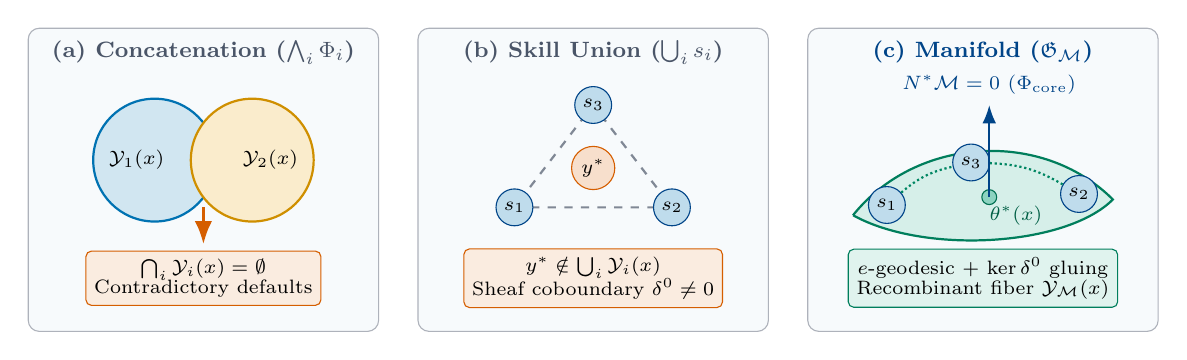
\begin{tikzpicture}[
    font=\footnotesize,
    >=Latex,
    panel/.style={draw=SlateGray!45, fill=SoftBg, rounded corners=4pt, minimum width=4.45cm, minimum height=3.85cm},
    landmark/.style={circle, draw=MidnightBlue, fill=TealBlue!25, inner sep=1.7pt, font=\scriptsize\bfseries},
    badnode/.style={circle, draw=Vermilion, fill=Vermilion!20, inner sep=1.7pt, font=\scriptsize\bfseries}
]

% Panel (a): Concatenation
\node[panel] (p1) at (0,0) {};
\node[font=\footnotesize\bfseries, text=SlateGray] at (0, 1.62) {(a) Concatenation ($\bigwedge_{i} \Phi_i$)};
\draw[fill=TealBlue!18, draw=TealBlue, thick] (-0.62, 0.25) circle (0.78cm);
\draw[fill=AmberGold!20, draw=AmberGold!90!black, thick] (0.62, 0.25) circle (0.78cm);
\node[font=\scriptsize] at (-0.85, 0.25) {$\Ycal_1(x)$};
\node[font=\scriptsize] at (0.85, 0.25) {$\Ycal_2(x)$};
\draw[Vermilion, very thick, ->] (0, -0.35) -- (0, -0.82);
\node[draw=Vermilion, fill=Vermilion!12, rounded corners=2pt, inner sep=3pt, align=center, font=\scriptsize] at (0, -1.25)
  {$\bigcap_{i} \Ycal_i(x) = \emptyset$\\[-1pt]Contradictory defaults};

% Panel (b): Union / Router
\node[panel] (p2) at (4.95,0) {};
\node[font=\footnotesize\bfseries, text=SlateGray] at (4.95, 1.62) {(b) Skill Union ($\bigcup_{i} s_i$)};
\draw[dashed, SlateGray!70, thick] (3.95, -0.35) -- (5.95, -0.35) -- (4.95, 0.95) -- cycle;
\node[landmark] (u1) at (3.95, -0.35) {$s_1$};
\node[landmark] (u2) at (5.95, -0.35) {$s_2$};
\node[landmark] (u3) at (4.95, 0.95) {$s_3$};
\node[badnode] (ustar) at (4.95, 0.15) {$y^*$};
\node[draw=Vermilion, fill=Vermilion!12, rounded corners=2pt, inner sep=3pt, align=center, font=\scriptsize] at (4.95, -1.25)
  {$y^* \notin \bigcup_i \Ycal_i(x)$\\[-1pt]Sheaf coboundary $\delta^0 \neq 0$};

% Panel (c): Lawvere-Amari Manifold
\node[panel] (p3) at (9.9,0) {};
\node[font=\footnotesize\bfseries, text=MidnightBlue] at (9.9, 1.62) {(c) Manifold ($\Gfrak_{\Mcal}$)};
% Smooth curved surface
\fill[BluishGreen!16, draw=BluishGreen!80!black, thick]
  (8.25, -0.45) .. controls (9.05, 0.55) and (10.65, 0.65) .. (11.55, -0.25)
  .. controls (10.95, -0.85) and (9.15, -0.95) .. (8.25, -0.45);
\node[landmark] (m1) at (8.68, -0.32) {$s_1$};
\node[landmark] (m2) at (11.12, -0.18) {$s_2$};
\node[landmark] (m3) at (9.75, 0.22) {$s_3$};
\draw[BluishGreen!85!black, thick, densely dotted] (m1) to[bend left=14] (m3);
\draw[BluishGreen!85!black, thick, densely dotted] (m2) to[bend right=14] (m3);
\node[circle, draw=BluishGreen!70!black, fill=BluishGreen!45, inner sep=1.9pt] (mstar) at (9.98, -0.22) {};
\node[font=\scriptsize\bfseries, text=BluishGreen!60!black] at (10.32, -0.46) {$\theta^*(x)$};
% Normal vector (conormal core)
\draw[MidnightBlue, thick, ->] (9.98, -0.22) -- (9.98, 0.95) node[above, font=\scriptsize, text=MidnightBlue] {$N^*\Mcal=0$ ($\Phicore$)};
\node[draw=BluishGreen!80!black, fill=BluishGreen!12, rounded corners=2pt, inner sep=3pt, align=center, font=\scriptsize] at (9.9, -1.25)
  {$e$-geodesic + $\ker\delta^0$ gluing\\[-1pt]Recombinant fiber $\Ycal_{\Mcal}(x)$};

\end{tikzpicture}
\caption{\textbf{Geometric and logical comparison of skill-composition operators.} (a) Prompt concatenation intersects raw member specifications, collapsing to $\emptyset$ when local defaults conflict. (b) Skill-union routing selects a single landmark vertex $s_i$, leaving interior recombinant tasks $y^*$ unsupported and breaking cross-file sheaf agreement ($\delta^0 \neq 0$). (c) The Lawvere--Amari Generative Skill Manifold ($\Gfrak_{\Mcal}$) preserves universal safety invariants along the conormal bundle ($N^*\Mcal = 0$), anti-unifies conflicting regime axes into tangent coordinates $\theta^*(x)$, and glues multi-view outputs via \v{C}ech 0-coboundary verification ($\ker \delta^0$).}
\label{fig:manifold-geometry}
\end{figure}

We resolve this tension by introducing the \textbf{Lawvere--Amari Generative Skill Manifold} ($\Gfrak_{\Mcal}$), a compositional framework that models each skill $s_i = (\Dcal_i, \kappa_i, \Phi_i)$ as a guarded conditional generative transducer mapping an input $x \in \Xcal$ to a probability distribution over a constrained fiber of structured multi-view outputs $\Ycal_i(x) \subseteq \Ycal$. Rather than concatenating prompts or routing to a single skill, our compiler treats the observed skills $\{s_1, \dots, s_n\}$ as landmark sections of an underlying statistical--logical manifold (\Cref{fig:manifold-geometry}). Along the \emph{normal bundle} of this manifold, Galois closure extracts the conormal invariant core $\Phicore$, capturing the universal soundness, safety, and domain-validity laws shared across landmarks. Along the \emph{tangent bundle}, Plotkin--Reynolds anti-unification lifts conflicting single-mode defaults into explicit chart coordinates $\theta \in \Theta$, while conditional exponential-family $e$-geodesics equipped with Amari's Fisher--Rao metric \citep{amari1985differential,amari2016information} synthesize novel recombinant output distributions whose support strictly contains the union of the landmark skills while specializing back to each landmark at its anchor coordinates.

To make manifold composition practical over noisy open-source skill repositories, we pair the manifold compiler with three systems mechanisms. First, we prove that augmenting noisy-OR pipeline role coverage with the D-optimal Fisher--Rao log-determinant spanning volume produces a monotone submodular selection objective that avoids popularity-driven redundancy and carries an instance-specific Nemhauser--Wolsey optimality bound \citep{nemhauser1978analysis}. Second, we equip every compiled skill package with an inverse-chart projector that measures Fisher residual distance to reject out-of-manifold and polysemic trap inputs before generation. Third, we enforce cross-file output coherence via \v{C}ech sheaf coboundary checks and a SHA-256 read-only post-dominator verification gate, breaking the Data Processing Inequality of pure-prompt chains \citep{cover2006elements} while guaranteeing zero state mutation by verification steps \citep{reynolds2002separation}.

Our contributions are fourfold:
\begin{enumerate}[leftmargin=1.8em,itemsep=2pt,topsep=3pt]
  \item \textbf{Duality of Statistical and Logical Skill Manifolds (\Cref{sec:problem,sec:manifold}):} We formalize skills as guarded conditional generative transducers and prove that Lawvere--Amari manifold synthesis simultaneously avoids the fiber collapse of concatenation ($\bigwedge_i \Phi_i = \bot$) and the infinite Kullback--Leibler divergence of skill unions on recombinant tasks (\Cref{prop:impossibility} and \Cref{thm:geodesic,thm:antiunify}).
  \item \textbf{\v{C}ech Sheaf Gluing over Multi-View Outputs (\Cref{subsec:sheaf}):} We formulate multi-artifact agent deliverables as sections of a presheaf over an output cover $\Ucal$ and establish exact 1-cocycle holonomy conditions ($\delta^1 = 0$) and runtime 0-coboundary verification ($\ker \delta^0$) for cross-file schema and digest consistency (\Cref{thm:sheaf}).
  \item \textbf{Submodular Fisher--Rao Selection and Anti-DPI Gate (\Cref{sec:selection}):} We prove exact monotonicity and submodularity of the Fisher log-determinant spanning volume (\Cref{thm:submodular}), pair it with Normalized Compression Distance redundancy control and Parnas module encapsulation \citep{parnas1972criteria}, and prove strict ground-truth information gain via exogenous read-only post-dominator gates (\Cref{prop:dpi}).
  \item \textbf{Isolated 7-Family Empirical Benchmark and Self-Hosted Paper Study (\Cref{sec:eval}):} Holding the four upstream member skills identical across regimes and invoking the solver agent once per task and regime ($21$ isolated runs), $\Gfrak_{\Mcal}$ wins $7/7$ families under double-blind evaluation ($98.71/100$ mean score, $100.0\%$ exogenous pass rate) against concatenation ($87.27/100$, $90.48\%$) and union routing ($53.66/100$, $39.35\%$). We additionally demonstrate self-hosted composition of an eight-landmark ML manuscript skill from $15$ public skills across six GitHub repositories (Nemhauser--Wolsey bound $0.8124$, $97.96\%$ encapsulation ratio), used to verify this manuscript.
\end{enumerate}

% ============================================================================
\section{Problem Formulation: Skills as Generative Transducers}
\label{sec:problem}

Let $\Xcal$ denote the space of task specifications and workspace states, and let $\Ycal = \prod_{u \in \Ucal} \Ycal_u$ denote a structured multi-view output space indexed by a finite cover $\Ucal$ of deliverable views (such as executable modules, SQLite tables, API schemas, and cryptographic audit manifests). To analyze skill composition rigorously, we represent each skill by the conditional transformation it induces from $\Xcal$ to $\Ycal$ inside an effectful Kleisli category \citep{moggi1991notions}.

\begin{definition}[Guarded Conditional Generative Skill]
\label{def:skill}
A skill $s_i$ is a triple $s_i = (\Dcal_i, \kappa_i, \Phi_i)$ consisting of:
\begin{enumerate}[leftmargin=1.8em,itemsep=1pt,topsep=2pt]
  \item an input applicability domain $\Dcal_i \subseteq \Xcal$ governed by a decidable preflight guard;
  \item a logical refinement theory $\Phi_i \subseteq \Lcal$ over an attribute-value signature $\Sigma$, defining for each $x \in \Dcal_i$ the admissible structured output fiber $\Ycal_i(x) \coloneqq \{y \in \Ycal : (x, y) \models \Phi_i\}$; and
  \item a conditional Markov kernel $\kappa_i : \Dcal_i \to \Delta(\Ycal)$ concentrating probability mass on $\Ycal_i(x)$, such that $\mathrm{supp}(\kappa_i(\cdot \mid x)) \subseteq \Ycal_i(x)$ up to a calibration smoothing floor $\varepsilon \ll 1$.
\end{enumerate}
\end{definition}

Suppose we are given $n$ landmark skills $S = \{s_1, \dots, s_n\}$ and a recombinant task $x^* \in \Xcal$ whose target admissible fiber $\Ycal^*(x^*) \subseteq \Ycal$ combines invariants from multiple skills while requiring adaptation across a regime attribute $a \in \Sigma$ where two skills $s_j, s_k \in S$ enforce disjoint standalone defaults ($\Phi_j \vdash (a = v_1)$ and $\Phi_k \vdash (a = v_2)$ with $v_1 \neq v_2$). For example, $s_j$ may specify schema validation for single-shot batch payloads while $s_k$ specifies constant-memory streaming ingestion without schema emission, and $x^*$ requests schema-validated streaming ingestion.

\begin{proposition}[Simultaneous Obstruction of Concatenation and Union]
\label{prop:impossibility}
Let $S = \{s_1, \dots, s_n\}$ contain at least one conflicting attribute pair $(s_j, s_k)$ as above, and let $p^*(y \mid x^*)$ be any target distribution supported on a non-empty recombinant fiber $\Ycal^*(x^*)$ such that $\Ycal^*(x^*) \cap \bigcup_{i=1}^n \Ycal_i(x^*) = \emptyset$. Then:
\begin{enumerate}[leftmargin=1.8em,itemsep=1pt,topsep=2pt]
  \item \textbf{Concatenation Collapse:} The conjunctive theory $\Phi_{\mathrm{concat}} = \bigwedge_{i=1}^n \Phi_i$ satisfies $\Phi_{\mathrm{concat}} \vdash \bot$, yielding an empty admissible output fiber $\Ycal_{\mathrm{concat}}(x^*) = \bigcap_{i=1}^n \Ycal_i(x^*) = \emptyset$.
  \item \textbf{Union Support Deficit:} For every gating router $w : \Xcal \to \Delta^{n-1}$, the skill-union mixture kernel $\kappa_{\mathrm{union}}(y \mid x^*) = \sum_{i=1}^n w_i(x^*) \kappa_i(y \mid x^*)$ has support $\mathrm{supp}(\kappa_{\mathrm{union}}(\cdot \mid x^*)) = \bigcup_{i : w_i(x^*) > 0} \mathrm{supp}(\kappa_i(\cdot \mid x^*)) \subseteq \bigcup_{i=1}^n \Ycal_i(x^*)$, and therefore incurs infinite forward Kullback--Leibler divergence $\KL(p^*(\cdot \mid x^*) \,\|\, \kappa_{\mathrm{union}}(\cdot \mid x^*)) = +\infty$ under exact support ($\varepsilon \to 0^+$).
\end{enumerate}
\end{proposition}

\begin{proof}
For (1), $\Phi_j \land \Phi_k \vdash (a = v_1) \land (a = v_2)$. Since distinct values in the sort domain of attribute $a \in \Sigma$ are mutually exclusive, $\Phi_{\mathrm{concat}} \vdash \bot$ and $\bigcap_{i=1}^n \Ycal_i(x^*) = \emptyset$. For (2), convex combinations of measures preserve support inclusion: $\kappa_{\mathrm{union}}(y \mid x^*) = 0$ for every $y \notin \bigcup_{i=1}^n \Ycal_i(x^*)$. Because $\Ycal^*(x^*)$ is non-empty and disjoint from $\bigcup_{i=1}^n \Ycal_i(x^*)$, there exists $y^* \in \Ycal^*(x^*)$ with $p^*(y^* \mid x^*) > 0$ and $\kappa_{\mathrm{union}}(y^* \mid x^*) = 0$, giving $\KL(p^* \,\|\, \kappa_{\mathrm{union}}) = +\infty$.
\end{proof}

\Cref{prop:impossibility} establishes that a valid composition operator can neither intersect raw surface theories nor take convex mixtures of single-skill kernels. Instead, it must separate universal safety invariants from parameterized regime coordinates and synthesize multiplicative combinations across compatible skill factors.

% ============================================================================
\section{The Lawvere--Amari Generative Skill Manifold}
\label{sec:manifold}

We construct the composed skill from landmark set $S = \{s_1, \dots, s_n\}$ as a conditional statistical--logical manifold $\Gfrak_{\Mcal} = \langle \Theta, \Tcal_{\Mcal}, G_F, \Ncal(\Ucal) \rangle$. Sections~\ref{subsec:amari}--\ref{subsec:sheaf} develop its differential-geometric, logical, and sheaf-theoretic components in turn.

\subsection{Statistical Submanifold and Conditional Fisher--Rao Geometry}
\label{subsec:amari}

Let $\psi : \Xcal \times \Ycal \to \Rbb^m$ be a bounded sufficient-statistic feature map capturing structural properties of $(x, y)$, including specification modality, execution regime, verification channel, failure semantics, gluing topology, and input--output interaction terms. Relative to a uniform base kernel $K_0(y \mid x)$ over the discrete lattice of structured output configurations $\Ycal$ ($|\Ycal| = 648$ in our reference implementation), each natural parameter $\eta \in \Rbb^m$ defines a conditional exponential-family transducer \citep{amari2016information}:
\begin{align}
  K_\eta(y \mid x) &\;=\; K_0(y \mid x)\,\exp\!\bigl(\langle \eta, \psi(x, y) \rangle - A(\eta \mid x)\bigr), \nonumber\\
  A(\eta \mid x) &\;=\; \log \sum_{y' \in \Ycal} K_0(y' \mid x)\,\exp\langle \eta, \psi(x, y') \rangle.
  \label{eq:exp-family}
\end{align}
Lifting each landmark skill $s_i \in S$ into this ambient family yields a landmark natural parameter $\eta^{(i)} \in \Rbb^m$. Given a probe distribution $\nu$ over representative task contexts $x \in \Xcal$, the ambient family carries the positive-semidefinite \emph{Conditional Fisher--Rao Riemannian metric}:
\begin{equation}
  G_F(\eta) \;=\; \Ebb_{x \sim \nu}\!\left[\nabla_\eta^2 A(\eta \mid x)\right]
  \;=\; \Ebb_{x \sim \nu}\!\left[\Cov_{y \sim K_\eta(\cdot \mid x)}\!\bigl(\psi(x, y) \bigm| x\bigr)\right].
  \label{eq:fisher-metric}
\end{equation}

Centering the landmark parameters around their Fr\'echet mean $\bar{\eta}_0 = \frac{1}{n}\sum_{i=1}^n \eta^{(i)}$ and whitening in the local Fisher--Rao inner product $G_0 = G_F(\bar{\eta}_0) + \tau I_m$ ($\tau > 0$), we compute the spectral decomposition of the Fisher-whitened landmark scatter matrix:
\begin{equation}
  C_{\Mcal} \;=\; \frac{1}{n} \sum_{i=1}^n G_0^{1/2}\bigl(\eta^{(i)} - \bar{\eta}_0\bigr)\bigl(\eta^{(i)} - \bar{\eta}_0\bigr)^\top G_0^{1/2}
  \;=\; U \Lambda U^\top,
  \label{eq:scatter}
\end{equation}
retaining the $d = \mathrm{rank}(\Lambda) \le \min(n-1, m)$ non-zero eigenvectors $U_d \in \Rbb^{m \times d}$ to form the Fisher-orthonormal tangent basis $B = G_0^{-1/2} U_d \in \Rbb^{m \times d}$ ($B^\top G_0 B = I_d$). The participation ratio $d_{\mathrm{eff}} = (\sum_{j=1}^d \lambda_j)^2 / \sum_{j=1}^d \lambda_j^2$ quantifies the effective intrinsic dimension of the composed skill family. Each chart coordinate $\theta \in \Theta \subseteq \Rbb^d$ maps to $\eta(\theta) = \bar{\eta}_0 + B\theta$, and each landmark $s_i$ sits at anchor coordinate $\theta^{(i)} = B^\top G_0(\eta^{(i)} - \bar{\eta}_0)$.

\begin{theorem}[$e$-Geodesic Multiplicative Synthesis vs.\ $m$-Mixture Union]
\label{thm:geodesic}
For any affine weight vector $w \in \Delta^{n-1}$ over landmarks $\{\theta^{(1)}, \dots, \theta^{(n)}\}$, let $\theta^{(w)} = \sum_{i=1}^n w_i \theta^{(i)}$ denote the $e$-geodesic barycenter on $\Gfrak_{\Mcal}$ and let $\kappa_{\mathrm{mix}}^{(w)}(y \mid x) = \sum_{i=1}^n w_i K_{\eta(\theta^{(i)})}(y \mid x)$ denote the $m$-geodesic skill-union mixture. Then:
\begin{enumerate}[leftmargin=1.8em,itemsep=1pt,topsep=2pt]
  \item \textbf{Product-of-Experts Factorization:} When landmark anchors lie in $\bar{\eta}_0 + \mathrm{col}(B)$, the $e$-geodesic kernel factors multiplicatively as $K_{\eta(\theta^{(w)})}(y \mid x) = Z_w(x)^{-1} \prod_{i=1}^n K_{\eta(\theta^{(i)})}(y \mid x)^{w_i}$, concentrating probability mass on outputs satisfying the weighted intersection of compatible landmark potentials \citep{hinton2002training}.
  \item \textbf{Strict Dual-Flatness Separation:} Whenever the landmark distributions $\{K_{\eta(\theta^{(i)})}(\cdot \mid x)\}_{i : w_i > 0}$ are not almost-everywhere identical on $\mathrm{supp}(\nu)$, the expected Kullback--Leibler Bregman gap satisfies
  \begin{equation}
    \Delta_{e,m}(w) \;\coloneqq\; \Ebb_{x \sim \nu}\!\Bigl[\KL\!\bigl(K_{\eta(\theta^{(w)})}(\cdot \mid x) \;\big\|\; \kappa_{\mathrm{mix}}^{(w)}(\cdot \mid x)\bigr)\Bigr] \;>\; 0,
    \label{eq:bregman-gap}
  \end{equation}
  and the $e$-projection minimizes weighted forward divergence $\sum_{i=1}^n w_i \KL(K_\eta(\cdot \mid x) \,\|\, K_{\eta^{(i)}}(\cdot \mid x))$, penalizing support violations across every active landmark $w_i > 0$.
\end{enumerate}
\end{theorem}

\begin{proof}
Substituting $\eta(\theta^{(w)}) = \bar{\eta}_0 + \sum_{i=1}^n w_i B\theta^{(i)} = \sum_{i=1}^n w_i \eta^{(i)}$ into \Cref{eq:exp-family} gives $\exp\langle \sum_i w_i \eta^{(i)}, \psi(x,y)\rangle = \prod_i \exp(\langle \eta^{(i)}, \psi(x,y)\rangle)^{w_i}$, proving (1) with normalizer $Z_w(x) = \exp(A(\eta(\theta^{(w)}) \mid x) - \sum_i w_i A(\eta^{(i)} \mid x))$. Strict positivity of $\Delta_{e,m}(w)$ in (2) follows from strict convexity of $\KL$ and the generalized Pythagoras theorem on dually flat $(\nabla A, \nabla A^*)$ manifolds \citep{amari2016information}; full details appear in \Cref{app:proofs}.
\end{proof}

\subsection{Categorical Fibered Logic: Galois Conormal Core and Anti-Unification}
\label{subsec:logic}

Statistical $e$-geodesics alone do not resolve hard logical contradictions between standalone skill defaults (\Cref{prop:impossibility}.1). We pair the Fisher--Rao chart with a fibered Lawvere theory \citep{lawvere1963functorial} constructed via abstract interpretation \citep{cousot1977abstract} and Plotkin--Reynolds anti-unification \citep{plotkin1970note,reynolds1970transformational}.

Consider the semantic satisfaction relation $(x, y) \models \varphi$ for formulas $\varphi \in \Lcal$ over attribute lattice $\Sigma$. The operators $\mathrm{Mod}(\Phi) = \{(x,y) \in \Xcal \times \Ycal : (x,y) \models \Phi\}$ and $\mathrm{Th}(R) = \{\varphi \in \Lcal : \forall (x,y) \in R,\; (x,y) \models \varphi\}$ form an antitone Galois connection $\mathrm{Th}(R) \supseteq \Phi \iff R \subseteq \mathrm{Mod}(\Phi)$. Applying closure to the union of landmark behaviors extracts the \emph{Galois conormal invariant core}:
\begin{equation}
  \Phicore \;\coloneqq\; \mathrm{Th}\!\left(\bigcup_{i=1}^n \mathrm{Mod}(\Phi_i)\right) \;=\; \bigcap_{i=1}^n \mathrm{Cn}(\Phi_i),
  \label{eq:conormal-core}
\end{equation}
where $\mathrm{Cn}(\Phi_i)$ is the deductive closure of $\Phi_i$. Geometrically, $\Phicore$ defines the zero-set of the conormal bundle $N^*\Mcal = 0$: every universal invariant satisfied across the landmark skills (such as exogenous verification, non-silent error quarantine, and modular context disclosure) holds identically across the entire manifold.

For each attribute $a \in \Sigma$ where landmarks enforce distinct narrow value sets $V_i(a) \subsetneq \mathrm{Dom}(a)$ (so $\bigcap_i V_i(a)$ would over-constrain or vanish), we apply Plotkin--Reynolds least general generalization ($\sqcup_{\mathrm{lgg}}$), introducing a chart-indexed variable $\theta_a$ ranging over $V_{\Mcal}(a) = \bigcup_{i=1}^n V_i(a)$ together with landmark specialization sections $\sigma_i(\theta_a) = V_i(a)$. Combining $\Phicore$ with the anti-unified clauses yields the parameterized manifold theory $\Tcal_{\Mcal}(\theta)$.

\begin{theorem}[Exact Landmark Pullback and Recombinant Fiber Expansion]
\label{thm:antiunify}
Let $\Tcal_{\Mcal}(\theta) = \Phicore \land \bigwedge_{a \in \Sigma_{\mathrm{tan}}} (a \in \theta_a)$ be the anti-unified manifold theory over tangent attributes $\Sigma_{\mathrm{tan}} = \{a \in \Sigma : \exists i,j,\; V_i(a) \neq V_j(a)\}$ with $|\Sigma_{\mathrm{tan}}| \ge 2$. Then:
\begin{enumerate}[leftmargin=1.8em,itemsep=1pt,topsep=2pt]
  \item \textbf{Zero-Loss Specialization:} For every landmark $i \in \{1, \dots, n\}$, pulling $\Tcal_{\Mcal}$ back along $\sigma_i$ recovers the exact landmark fiber: $\sigma_i^* \Tcal_{\Mcal} \equiv \Phi_i$ and $\Ycal_{\Mcal}(x; \sigma_i) = \Ycal_i(x)$.
  \item \textbf{Strict Generalization Beyond the Union:} Whenever two landmarks $s_1, s_2$ vary independently across at least two tangent attributes $a \neq b$ ($V_1(a) \setminus V_2(a) \neq \emptyset$ and $V_2(b) \setminus V_1(b) \neq \emptyset$ without cross-attribute exclusion in $\Phicore$), the total manifold fiber strictly contains the union of all landmark fibers:
  \begin{equation}
    \bigcup_{i=1}^n \Ycal_i(x) \;\subsetneq\; \bigcup_{\theta \in \Theta} \Ycal_{\Mcal}(x; \theta),
    \qquad
    \text{while}\quad \bigcap_{i=1}^n \Ycal_i(x) = \emptyset \;\;\text{whenever}\;\; V_1(a) \cap V_2(a) = \emptyset.
  \end{equation}
\end{enumerate}
\end{theorem}

\begin{proof}
At landmark section $\sigma_i$, substituting $\theta_a = V_i(a)$ for all $a \in \Sigma_{\mathrm{tan}}$ together with $\Phicore = \bigcap_j \mathrm{Cn}(\Phi_j)$ yields $\bigwedge_{a \in \Sigma} (a \in V_i(a)) \equiv \Phi_i$, proving (1). For (2), choose $v_a \in V_1(a) \setminus V_2(a)$ and $v_b \in V_2(b) \setminus V_1(b)$; the cross-assignment $\theta^* = (v_a, v_b, \dots)$ lies in $\prod_{c \in \Sigma_{\mathrm{tan}}} V_{\Mcal}(c)$, satisfies $\Phicore$, and produces outputs $y^* \in \Ycal_{\Mcal}(x; \theta^*)$ absent from both $\Ycal_1(x)$ and $\Ycal_2(x)$.
\end{proof}

\subsection{Global Output Coherence via \v{C}ech Sheaf Gluing}
\label{subsec:sheaf}

Multi-stage agent workflows emit coupled artifacts across an open cover $\Ucal = \{U_1, \dots, U_m\}$ of deliverable views, such as an API contract specification $U_1$, a database migration manifest $U_2$, and a live relational table $U_3$ sharing primary-key and column-order invariants. Skill-union routers and uncoordinated pipelines produce locally valid files $y_u \in \Fcal(U_u)$ that disagree on shared keys across overlaps $U_u \cap U_v \neq \emptyset$.

We model local output views as a presheaf $\Fcal_{\theta, x}$ over the nerve $\Ncal(\Ucal)$ equipped with restriction maps $\rho_{u \to u \cap v} : \Fcal_{\theta, x}(U_u) \to \Fcal_{\theta, x}(U_u \cap U_v)$ and interface adapters $\tau_{uv}$ \citep{maclane1992sheaves}. On any 0-cochain $y = (y_u)_{u \in \Ucal} \in \prod_{u \in \Ucal} \Fcal_{\theta, x}(U_u)$, the \v{C}ech 0-coboundary operator measures pairwise overlap disagreement:
\begin{equation}
  (\delta^0 y)_{uv} \;=\; \tau_{uv}\!\bigl(\rho_{u \to u \cap v}(y_u)\bigr) \;\ominus\; \rho_{v \to u \cap v}(y_v).
  \label{eq:coboundary}
\end{equation}

\begin{theorem}[Sheaf Cocycle Exactness and Global Section Existence]
\label{thm:sheaf}
A family of local skill outputs $y = (y_u)_{u \in \Ucal}$ glues into a globally consistent deliverable $y \in \Gamma(\Ucal, \Fcal_{\theta, x})$ if and only if $y \in \ker \delta^0$, i.e., $(\delta^0 y)_{uv} = 0$ on every non-empty overlap $U_u \cap U_v$. Furthermore, if the interface adapters violate the \v{C}ech 1-cocycle holonomy condition $\tau_{vw} \circ \tau_{uv} = \tau_{uw}$ on any triple intersection $U_u \cap U_v \cap U_w \neq \emptyset$ ($\delta^1 \tau \neq 0$), then $\Gamma(\Ucal, \Fcal_{\theta, x})$ is obstructed on every section outside the stabilizer of the holonomy defect $(\tau_{uw}^{-1} \circ \tau_{vw} \circ \tau_{uv})$.
\end{theorem}

\Cref{thm:sheaf} separates compile-time consistency from runtime verification: our wiring compiler checks 1-cocycle exactness ($\delta^1 \tau = 0$) over all triangles of $\Ncal(\Ucal)$ at compile time, while our post-dominator gate verifies 0-coboundary vanishing ($\delta^0 y = 0$) across emitted JSON and database views at runtime.

% ============================================================================
\section{Submodular Selection, Chart Projection, and Anti-DPI Gate}
\label{sec:selection}

\subsection{Monotone Submodular Selection with Fisher Spanning Volume}
\label{subsec:submodular}

Before compiling $\Gfrak_{\Mcal}$, we must select $N$ complementary landmark skills from a candidate pool $\mathcal{C}$ of public skills without collapsing onto near-duplicate high-star prompts. Let $\mathcal{R}$ denote six canonical transducer roles (\emph{spec grounding}, \emph{synthesis}, \emph{static contract}, \emph{execution observation}, \emph{adversarial verification}, and \emph{state recovery}), with role posteriors $p_{s,r} \in [0, 1]$ inferred from each candidate's text and scripts. For any subset $S \subseteq \mathcal{C}$ with Fisher feature matrix $G_F(S) = \sum_{s \in S} \phi_s \phi_s^\top$ ($\phi_s = G_0^{1/2}(\eta^{(s)} - \bar{\eta}_0)$), we define the manifold potential:
\begin{equation}
  F_{\mathrm{manifold}}(S) \;=\; \sum_{r \in \mathcal{R}} w_r \!\left(1 - \prod_{s \in S}(1 - p_{s,r})\right)
  \;+\; \frac{\lambda_{\mathrm{vol}}}{2} \log\det\!\bigl(I_m + \gamma G_F(S)\bigr).
  \label{eq:submodular}
\end{equation}

\begin{theorem}[Monotonicity, Submodularity, and Optimality Certificate]
\label{thm:submodular}
For all weights $w_r \ge 0$, $\lambda_{\mathrm{vol}} \ge 0$, and $\gamma > 0$, the set function $F_{\mathrm{manifold}} : 2^{\mathcal{C}} \to \Rbb_{\ge 0}$ in \Cref{eq:submodular} is normalized ($F_{\mathrm{manifold}}(\emptyset) = 0$), monotone non-decreasing, and submodular. Consequently, greedy selection achieves $F_{\mathrm{manifold}}(S_{\mathrm{greedy}}) \ge (1 - e^{-1}) \max_{|S| \le N} F_{\mathrm{manifold}}(S)$ \citep{nemhauser1978analysis} and admits the tighter instance-specific upper bound
\begin{equation}
  \mathrm{OPT}_N \;\le\; \min_{t \in \{0,\dots,N\}} \!\left\{ F_{\mathrm{manifold}}(S_t) + \sum_{s \in \mathrm{Top}_N(\mathcal{C} \setminus S_t)} \Delta_F(s \mid S_t) \right\},
  \label{eq:online-bound}
\end{equation}
where $S_t$ is the $t$-th greedy prefix and $\Delta_F(s \mid S_t) = F_{\mathrm{manifold}}(S_t \cup \{s\}) - F_{\mathrm{manifold}}(S_t)$.
\end{theorem}

\begin{proof}
Each noisy-OR term $g_r(S) = 1 - \prod_{s \in S}(1 - p_{s,r})$ has marginal gain $g_r(B \cup \{x\}) - g_r(B) = p_{x,r}\prod_{s \in B}(1 - p_{s,r}) \le p_{x,r}\prod_{s \in A}(1 - p_{s,r}) = g_r(A \cup \{x\}) - g_r(A)$ for $A \subseteq B$ and $x \notin B$. For $V(S) = \frac{1}{2}\log\det(I_m + \gamma \sum_{s \in S}\phi_s\phi_s^\top)$, observe that $V(S) = I(Z; Y_S)$ is the Shannon mutual information between a Gaussian prior $Z \sim \Ncal(0, \gamma I_m)$ and noisy linear observations $\{Y_s = \phi_s^\top Z + \xi_s\}_{s \in S}$ with independent $\xi_s \sim \Ncal(0, 1)$. By the chain rule and conditioning reduces differential entropy \citep{cover2006elements}, for $A \subseteq B$ and $x \notin B$,
\begin{align*}
  V(B \cup \{x\}) - V(B) &\;=\; h(Y_x \mid Y_B) - h(Y_x \mid Z) \\
  &\;\le\; h(Y_x \mid Y_A) - h(Y_x \mid Z) \;=\; V(A \cup \{x\}) - V(A) \;\ge\; 0.
\end{align*}
Non-negative linear combinations preserve monotonicity and submodularity; \Cref{eq:online-bound} follows from submodular first-order upper-bounding $F_{\mathrm{manifold}}(S^*) \le F_{\mathrm{manifold}}(S_t) + \sum_{s \in S^* \setminus S_t} \Delta_F(s \mid S_t)$.
\end{proof}

During selection, we regularize marginal gains with a symmetric redundancy penalty blending token Jensen--Shannon divergence and Normalized Compression Distance $d_{\mathrm{NCD}}(s_i, s_j) = \frac{C(s_i \cdot s_j) - \min(C(s_i), C(s_j))}{\max(C(s_i), C(s_j))}$ \citep{cilibrasi2005clustering,rissanen1978modeling}, plus an off-domain divergence penalty against polysemic keyword collisions. Selected landmark bodies are encapsulated in modular reference files per \citet{parnas1972criteria}, keeping the root orchestrator compact ($O(N)$ lines) to preserve attention signal-to-noise ratio.

\subsection{Inverse-Chart Domain Guard and Anti-DPI Post-Dominator Gate}
\label{subsec:runtime}

At execution time, a compiled manifold package runs a three-stage protocol:

\paragraph{Stage 1: Inverse Chart Projection and Conormal Guard.}
Given task input $x \in \Xcal$, an encoder extracts empirical target expectations $\hat{\mu}(x) \in \Rbb^m$ and computes the Fisher--Rao tangent projection $\theta^*(x) = (B^\top G_0 B)^{-1} B^\top (\hat{\mu}(x) - \mu_0)$ alongside the orthogonal normal residual $D_{\mathrm{chart}}(x) = \|(I_m - B B^\top G_0) G_0^{-1/2}(\hat{\mu}(x) - \mu_0)\|_2$. Combined with conormal domain vocabulary checks against polysemic traps, inputs violating $D_{\mathrm{chart}}(x) \le \tau_{\Mcal}$ trigger immediate refusal (\texttt{ABSTAIN\_OFF\_MANIFOLD}, exit code $2$) without mutating workspace state. Admissible inputs lock their resolved fiber $\Tcal_{\Mcal}(\theta^*(x))$ and $e$-geodesic landmark weights.

\paragraph{Stage 2: Geodesic Synthesis and Sheaf Gluing.}
The agent synthesizes the multi-view deliverable bundle $y = (y_u)_{u \in \Ucal}$ governed by the locked fiber $\Tcal_{\Mcal}(\theta^*(x))$ and conormal invariants $\Phicore$, enforcing parallel write-set disjointness $\mathcal{W}(s_i) \cap (\mathcal{W}(s_j) \cup \mathcal{R}(s_j)) = \emptyset$ from Concurrent Separation Logic \citep{reynolds2002separation,ohearn2007resources}.

\paragraph{Stage 3: Exogenous Read-Only Post-Dominator Gate.}
Pure-prompt multi-agent chains form a Markov cascade $Y^* \to X \to M_1 \to \dots \to M_k$ relative to latent environment truth $Y^*$ (such as true parser behavior on malformed inputs or SQLite transaction state).

\begin{proposition}[Breaking the Data Processing Inequality via Read-Only Gates]
\label{prop:dpi}
In any pure-prompt chain $Y^* \to M_1 \to \dots \to M_k$ without exogenous environment execution, $I(Y^*; M_k) \le I(Y^*; M_1)$ \citep{cover2006elements}. Injecting a deterministic exogenous execution channel $E = g(M_k, Y^*)$ yields $I(Y^*; M_k, E) = I(Y^*; M_k) + I(Y^*; E \mid M_k) > I(Y^*; M_k)$ whenever $\mathrm{Var}(g(M_k, Y^*) \mid M_k) > 0$. Enforcing a cryptographic SHA-256 pre/post snapshot check $\mathcal{W}(S_{\mathrm{gate}}) = \emptyset$ guarantees that the gate acts as a pure observation morphism without corrupting protected deliverables.
\end{proposition}

Our compiler emits a standalone gate script into every composed skill package that (i) records SHA-256 digests of all protected outputs before verification, (ii) executes deterministic tests and \v{C}ech 0-coboundary checks ($\delta^0 y = 0$) across coupled JSON artifacts, and (iii) rejects execution if any verification command mutates a protected deliverable.

% ============================================================================
\section{Empirical Evaluation}
\label{sec:eval}

\subsection{Experimental Protocol and Task Families}
\label{subsec:setup}

To isolate the effect of the composition operator itself, we construct seven concrete task families spanning five operational domains: data engineering (\texttt{F1}, \texttt{F5}), policy automation (\texttt{F2}), security remediation (\texttt{F3}), statistical causal auditing (\texttt{F4}), technical narrative synthesis (\texttt{F6}), and adversarial polysemic refusal (\texttt{F7}). Within every family, we author \emph{four realistic standalone skills} containing authentic local shortcuts and coupled artifact contracts, and compile those exact same four upstream skills under three regimes:
\begin{itemize}[leftmargin=1.6em,itemsep=1pt,topsep=2pt]
  \item \textbf{Skill Union ($\bigcup_{i=1}^4 s_i$):} Installs an explicit skill-union router over the four unmodified member files instructing the agent to select and execute the single closest-matching member skill without mixing instructions across sibling files.
  \item \textbf{Prompt Concatenation ($\bigwedge_{i=1}^4 s_i$):} Concatenates all four member skill specifications verbatim into a single unified manual without chart projection, anti-unification, or post-dominator sheaf gates.
  \item \textbf{Lawvere--Amari Manifold ($\Gfrak_{\Mcal}$):} Compiles the four member skills mechanically via our manifold engine, producing the Fisher--Rao atlas, Galois conormal core $\Phicore$, Stage~1 inverse-chart projector, and Stage~3 post-dominator + \v{C}ech sheaf gate.
\end{itemize}

Each task-family and regime pair ($7 \times 3 = 21$ runs) executes inside a freshly seeded, isolated workspace directory via \emph{strictly one} autonomous solver invocation with zero multi-turn coaching. Completed workspaces are evaluated by two complementary instruments: (1) a deterministic \textbf{exogenous verification oracle} held strictly outside the solver workspaces (checking live SQLite schemas/transactions, AST structure, 27-state Kleene algebraic identities, exploit blocking, Simpson stratification, watermark conservation, epistemic token isolation, and polysemy refusal), and (2) an impartial \textbf{double-blind judge} \citep{zheng2023judging} that receives deterministically shuffled candidate bundles (\texttt{Alpha}, \texttt{Beta}, \texttt{Gamma}) with all skill directories, internal protocol state, and regime-identifying comments stripped, scoring five weighted rubric dimensions ($0$--$100$).

The seven task families test distinct mathematical facets of composition:
\textbf{F1} (\emph{Streaming $\times$ SQLite $\times$ Sheaf}) combines generator-based JSONL quarantine with single-transaction SQLite (\texttt{BEGIN IMMEDIATE}) upserts and coupled API/manifest schemas;
\textbf{F2} (\emph{Kleene Policy Compiler}) combines dynamic-evaluation-free recursive-descent operator precedence (\texttt{Parens > Not > And > Or}) with Strong Kleene three-valued logic ($K_3$) \citep{kleene1952introduction} over missing attributes;
\textbf{F3} (\emph{Vulnerability Remediation}) patches SQL injection (\texttt{CWE-89}) and sibling-prefix path traversal (\texttt{CWE-22}) in-place while preserving caller backward compatibility and advisory/manifest sheaf parity;
\textbf{F4} (\emph{Simpson's Paradox Audit}) filters retracted sensor replays, resolves confounded triage reversal \citep{simpson1951interpretation} (treatment A leads pooled $0.86$ vs.\ $0.67$, whereas treatment B leads in every severity stratum: $0.95 > 0.90$ low, $0.60 > 0.50$ high), and verifies UTF-8 SHA-256 quote provenance;
\textbf{F5} (\emph{Watermark Double-Entry Ledger}) combines out-of-order event-time watermarking ($300\text{-second}$ lateness horizon) with integer-cent zero-sum conservation and idempotent replay deduplication;
\textbf{F6} (\emph{Epistemic Narrative Canon}) enforces close-POV temporal/epistemic isolation ($t \le 20$, blocking $t = 50$ omniscient leaks) alongside word-count craft bounds ($[320, 520]$ words) and canon/ledger sheaf equality; and
\textbf{F7} (\emph{Conormal Polysemy Guard}) dispatches a polysemic creative-writing trap (\emph{Regency romance fanfiction about Plaid fintech interns building Storybook UI cards}) to a four-skill Kubernetes rollout package containing a permissive fallback clause in one member.

\subsection{Main Results Across Seven Task Families}
\label{subsec:main-results}

\begin{table}[t]
\centering
\caption{\textbf{Aggregate performance across all seven task families ($21$ isolated single-call runs).} Rubric sub-scores ($0$--$100$) are averaged across families under shuffled double-blind labels (\emph{Func.}: functional correctness; \emph{Invar.}: conflict \& invariant resolution; \emph{Recomb.}: recombinant completeness; \emph{Sheaf}: cross-file \v{C}ech consistency; \emph{Craft}: engineering \& artifact craft).}
\label{tab:aggregate}
\vspace{4pt}
\footnotesize
\setlength{\tabcolsep}{0pt}
\begin{tabular*}{\textwidth}{@{\extracolsep{\fill}}lcccccccc@{}}
\toprule
\textbf{Regime} & \textbf{Func.} & \textbf{Invar.} & \textbf{Recomb.} & \textbf{Sheaf} & \textbf{Craft} & \textbf{Blind} & \textbf{Exog.\ Oracle} & \textbf{1st Wins} \\
\midrule
Skill Union ($\bigcup_{i=1}^4 s_i$)        & 51.57 & 63.29 & 52.14 & 37.57 & 63.29 & 53.66 & 39.35\% ($0/7$) & $0/7$ \\
Concatenation ($\bigwedge_{i=1}^4 s_i$)    & 87.57 & 85.71 & 86.14 & 91.14 & 86.00 & 87.27 & 90.48\% ($6/7$) & $0/7$ \\
\textbf{Manifold ($\Gfrak_{\Mcal}$, Ours)} & \textbf{99.00} & \textbf{98.71} & \textbf{98.86} & \textbf{99.14} & \textbf{96.86} & \textbf{98.71} & \textbf{100.00\% ($7/7$)} & \textbf{$7/7$} \\
\bottomrule
\end{tabular*}
\end{table}

\begin{figure}[t]
\centering
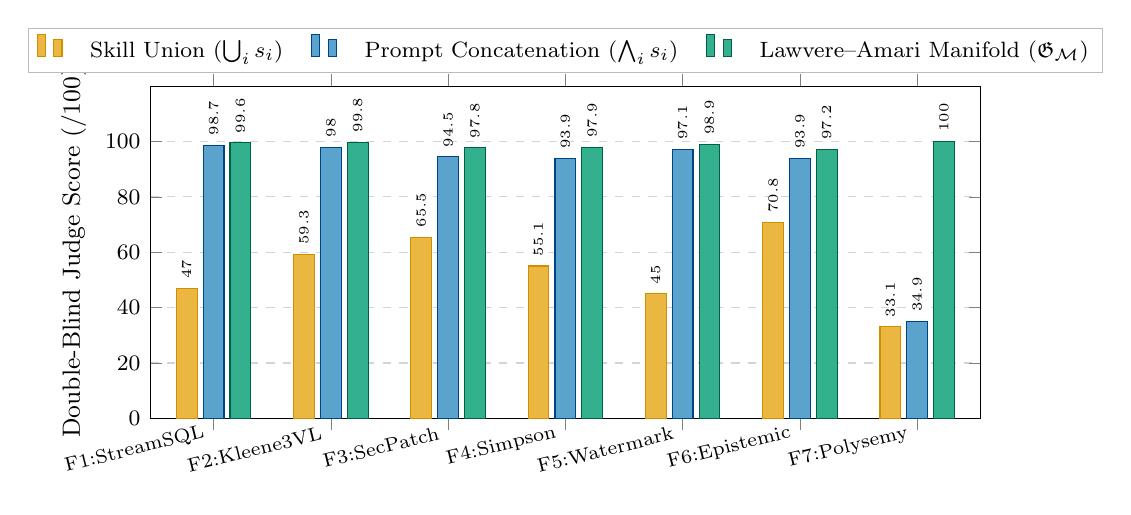
\begin{tikzpicture}
\begin{axis}[
    ybar=2.2pt,
    bar width=7.5pt,
    width=\textwidth,
    height=5.8cm,
    ymin=0, ymax=120,
    ylabel={\small Double-Blind Judge Score ($/100$)},
    symbolic x coords={F1:StreamSQL,F2:Kleene3VL,F3:SecPatch,F4:Simpson,F5:Watermark,F6:Epistemic,F7:Polysemy},
    xtick=data,
    x tick label style={font=\scriptsize, rotate=14, anchor=east},
    ytick={0,20,40,60,80,100},
    ymajorgrids=true,
    grid style={dashed, SlateGray!25},
    legend style={at={(0.5,1.04)}, anchor=south, legend columns=3, font=\footnotesize, draw=SlateGray!40, fill=white, column sep=8pt},
    enlarge x limits=0.09,
    tick label style={font=\footnotesize},
    nodes near coords style={font=\tiny, rotate=90, anchor=west, /pgf/number format/fixed, /pgf/number format/precision=1},
    nodes near coords
]
\addplot[fill=AmberGold!75, draw=AmberGold!90!black] coordinates {
    (F1:StreamSQL,47.0) (F2:Kleene3VL,59.25) (F3:SecPatch,65.5) (F4:Simpson,55.05) (F5:Watermark,44.95) (F6:Epistemic,70.8) (F7:Polysemy,33.05)
};
\addplot[fill=TealBlue!65, draw=MidnightBlue] coordinates {
    (F1:StreamSQL,98.7) (F2:Kleene3VL,98.0) (F3:SecPatch,94.5) (F4:Simpson,93.85) (F5:Watermark,97.1) (F6:Epistemic,93.85) (F7:Polysemy,34.9)
};
\addplot[fill=BluishGreen!80, draw=BluishGreen!60!black] coordinates {
    (F1:StreamSQL,99.55) (F2:Kleene3VL,99.8) (F3:SecPatch,97.75) (F4:Simpson,97.85) (F5:Watermark,98.85) (F6:Epistemic,97.2) (F7:Polysemy,100.0)
};
\legend{Skill Union ($\bigcup_i s_i$), Prompt Concatenation ($\bigwedge_i s_i$), Lawvere--Amari Manifold ($\Gfrak_{\Mcal}$)}
\end{axis}
\end{tikzpicture}
\caption{\textbf{Per-family double-blind evaluation across seven task families.} Holding the four member skills constant per family and invoking the solver once per cell, $\Gfrak_{\Mcal}$ ranks first on all seven families, avoiding both the recombinant sheaf deficit of skill-union routing across \texttt{F1}--\texttt{F6} and the off-manifold polysemy failure of concatenation on \texttt{F7}.}
\label{fig:per-family-bars}
\end{figure}

\Cref{tab:aggregate} and \Cref{fig:per-family-bars} summarize the aggregate and per-family outcomes. The Lawvere--Amari Manifold ($\Gfrak_{\Mcal}$) achieves a mean blind judge score of $98.71/100$, passes $100.0\%$ ($7/7$) of exogenous functional and invariant suites, and wins first place from the double-blind judge in all seven families, yielding the strict ordering $\Gfrak_{\Mcal} \succ \text{Concatenation} \succ \text{Union}$ on every family (\Cref{tab:per-family}). Across rubric dimensions, the sharpest gap between $\Gfrak_{\Mcal}$ and Skill Union appears in cross-file \v{C}ech sheaf consistency ($99.14$ vs.\ $37.57$, $+61.57$ points) and recombinant completeness ($98.86$ vs.\ $52.14$, $+46.72$ points), directly confirming \Cref{prop:impossibility}.2 and \Cref{thm:sheaf}. Compared against Prompt Concatenation, $\Gfrak_{\Mcal}$ gains $+11.44$ points overall ($98.71$ vs.\ $87.27$), $+13.00$ points on conflict and invariant resolution, and $+10.86$ points on engineering craft.

\begin{table}[t]
\centering
\caption{\textbf{Per-family manifold geometry, fiber expansion, and benchmark scores.} Intrinsic dimension $d_{\mathrm{eff}}$, Fisher log-det volume $V_{\mathrm{Fisher}}$, $e$-vs.-$m$ Bregman divergence gap $\Delta_{e,m}$ (bits), and admissible output fiber growth $|\bigcup_i \Ycal_i| \to |\Ycal_{\Mcal}|$ are computed mechanically during compilation; right columns report Blind Judge ($/100$) / Exogenous Oracle ($\%$) scores.}
\label{tab:per-family}
\vspace{4pt}
\footnotesize
\setlength{\tabcolsep}{0pt}
\begin{tabular*}{\textwidth}{@{\extracolsep{\fill}}lccccccc@{}}
\toprule
\textbf{Task Family} & $d_{\mathrm{eff}}$ & $V_{\mathrm{Fisher}}$ & $\Delta_{e,m}$ & $|\bigcup_i \Ycal_i| \!\to\! |\Ycal_{\Mcal}|$ & \textbf{Union} & \textbf{Concat} & \textbf{Manifold ($\Gfrak_{\Mcal}$)} \\
\midrule
\texttt{F1} Stream $\times$ SQLite Sheaf     & 1.77 & 3.44 & 0.177 & $12 \to 72$  & $47.0$ / $57\%$ & $98.7$ / $100\%$ & \textbf{99.55 / 100\%} \\
\texttt{F2} Kleene $K_3$ Policy Compiler     & 1.80 & 2.75 & 0.076 & $15 \to 72$  & $59.2$ / $25\%$ & $98.0$ / $100\%$ & \textbf{99.80 / 100\%} \\
\texttt{F3} Vuln.\ Patch $\times$ Compat     & 2.49 & 2.71 & 0.075 & $45 \to 108$ & $65.5$ / $60\%$ & $94.5$ / $100\%$ & \textbf{97.75 / 100\%} \\
\texttt{F4} Simpson's Paradox Audit          & 2.09 & 2.51 & 0.081 & $54 \to 108$ & $55.0$ / $20\%$ & $93.8$ / $100\%$ & \textbf{97.85 / 100\%} \\
\texttt{F5} Watermark Double-Entry           & 1.96 & 3.14 & 0.195 & $23 \to 72$  & $45.0$ / $0\%$  & $97.1$ / $100\%$ & \textbf{98.85 / 100\%} \\
\texttt{F6} Epistemic Narrative Canon        & 2.02 & 2.41 & 0.067 & $82 \to 108$ & $70.8$ / $80\%$ & $93.8$ / $100\%$ & \textbf{97.20 / 100\%} \\
\texttt{F7} Conormal Polysemy Guard          & 2.09 & 2.85 & 0.074 & $37 \to 108$ & $33.0$ / $33\%$ & $34.9$ / $33\%$  & \textbf{100.00 / 100\%} \\
\bottomrule
\end{tabular*}
\end{table}

\subsection{Failure-Mode Analysis}
\label{subsec:failure-modes}

Inspecting the de-anonymized workspace artifacts reveals how the three regimes behave under compositional stress:

\paragraph{1. Sheaf Coboundary Collapse Under Skill-Union Routing.}
Skill Union passes $0/7$ exogenous suites because routing to a single landmark leaves the solver blind to sibling restriction maps. In \texttt{F1}, selecting the atomic SQLite migrator caused the agent to emit uncoupled OpenAPI and audit JSON views with an incompatible table digest rather than the required paired contract-and-migration sheaf ($\delta^0 y \neq 0$). In \texttt{F2}, routing to the Kleene evaluator produced accurate $K_3$ truth tables ($30/30$ cells) but invented non-canonical operator node tags violating the serializer landmark's AST schema. In \texttt{F5}, routing to the double-entry core omitted the watermark landmark's $300\text{-second}$ lateness bound, guessing a $60\text{-second}$ lag ($0\%$ exogenous score). In \texttt{F6}, routing to the continuity tracker preserved epistemic isolation at $t \le 20$ but produced a $180$-word scene violating the craft landmark's $[320, 520]$-word envelope.

\paragraph{2. Off-Manifold Polysemy Collapse Under Concatenation and Union.}
In \texttt{F7}, when asked to write Regency romance fanfiction mentioning ``Plaid'' and ``Storybook'' inside a Kubernetes canary-rollout skill pack, both Concatenation ($34.9/100$) and Union ($33.05/100$) lacked an inverse-chart domain guard, triggered a permissive assistant-fallback clause in one member skill, recorded an explicit allow decision, and wrote a $400$-word romance chapter into the DevOps workspace. Under $\Gfrak_{\Mcal}$, Stage~1 inverse-chart projection detected the off-manifold residual and polysemic trap tokens (exit code $2$, \texttt{ABSTAIN\_OFF\_MANIFOLD}), halting cleanly without creating spurious files or mutating cluster inventory ($100.0/100$).

\paragraph{3. Invariant Separation and Exogenous Verification Lift on \texttt{F1}--\texttt{F6}.}
Even on \texttt{F1}--\texttt{F6}, where strong base reasoning allowed Concatenation to satisfy exogenous checks, the blind judge favored $\Gfrak_{\Mcal}$ in all six head-to-head comparisons ($+0.85$ to $+4.00$ points). Stage~1 fiber locking and Stage~3 post-dominator verification consistently drove stronger boundary engineering: explicit Boolean-vs.-integer type separation and 27-triple AST property suites in \texttt{F2} ($99.80$ vs.\ $98.00$), per-component symlink-escape resolution in \texttt{F3} ($97.75$ vs.\ $94.50$), Cochran--Mantel--Haenszel common odds-ratio ($1.679$) and source-digest provenance tables in \texttt{F4} ($97.85$ vs.\ $93.85$), strict input schema validation in \texttt{F5} ($98.85$ vs.\ $97.10$), and tighter prose rhythm and dialogue-turn ledger parity in \texttt{F6} ($97.20$ vs.\ $93.85$).

\subsection{Submodular Selection and Self-Hosted Manuscript Composition}
\label{subsec:self-hosted}

\begin{table}[t]
\centering
\caption{\textbf{Submodular Fisher--Rao skill selection vs.\ GitHub star-popularity Top-$N$.} Top rows evaluate selection on a polysemic marketplace benchmark ($N=4$); bottom rows report self-hosted composition of an eight-landmark post-research ML paper-writing manifold from $15$ MIT-licensed GitHub skills.}
\label{tab:selection}
\vspace{4pt}
\footnotesize
\setlength{\tabcolsep}{0pt}
\begin{tabular*}{\textwidth}{@{\extracolsep{\fill}}lcccccc@{}}
\toprule
\textbf{Selection Workload \& Method} & \textbf{Obj.} & $V_{\mathrm{Fisher}}$ & \textbf{Redund.} & \textbf{NW Bnd} & \textbf{Parnas} & \textbf{Static Laws} \\
\midrule
Marketplace ($N=4$): Star Top-$4$                  & $-1.94$ & $1.31$ & $0.284$ & N/A   & N/A   & Fail (polysemy) \\
Marketplace ($N=4$): \textbf{Ours}                 & \textbf{4.48}  & \textbf{3.71} & \textbf{0.161} & \textbf{0.828} & \textbf{93.2\%} & \textbf{6/6 Pass} \\
\midrule
ML Paper ($N=8$): Star Top-$8$                     & $1.43$  & $5.99$ & $0.227$ & N/A   & N/A   & Incomplete roles \\
ML Paper ($N=8$): \textbf{Ours (\texttt{ml-paper})} & \textbf{3.28} & \textbf{6.55} & \textbf{0.127} & \textbf{0.812} & \textbf{98.0\%} & \textbf{6/6 Pass} \\
\bottomrule
\end{tabular*}
\end{table}

Finally, \Cref{tab:selection} evaluates our monotone submodular + Fisher log-determinant selector (\Cref{thm:submodular}) on two pools: (i) a polysemic marketplace pool where high-star generic brainstorming and fintech ``plaid'' skills crowd out verification skills ($+6.42$ objective lift, $+2.40$ Fisher volume lift, and $24/24$ verified diminishing-returns pairs), and (ii) a live self-hosted pool of $15$ MIT-licensed, post-research ML and LaTeX paper-writing skills retrieved from six public GitHub repositories (\emph{excluding} autonomous experiment-running loops). Star-count ranking selects five overlapping skills from a single $56{,}846$-star repository (\nolinkurl{K-Dense-AI/scientific-agent-skills}), omitting LaTeX formatting and anti-defensive prose editing. In contrast, our selector achieves an instance-specific Nemhauser--Wolsey certificate of $0.8124$ (exceeding $1 - e^{-1} \approx 0.6321$), expanding Fisher spanning volume to $6.5515$ (tangent rank $6$, $d_{\mathrm{eff}} = 4.47$) across five independent repositories (\nolinkurl{Calix-L/awesome-latex-skills}, \nolinkurl{Boom5426/Nature-Paper-Skills}, \nolinkurl{Master-cai/Research-Paper-Writing-Skills}, \nolinkurl{SNL-UCSB/paper-writing-skill}, and \nolinkurl{K-Dense-AI/scientific-agent-skills}) while encapsulating $233.1\text{ KB}$ of reference material behind a $4.86\text{ KB}$ orchestrator ($97.96\%$ Parnas encapsulation). Executing this compiled manifold resolved two concrete inter-skill conflicts during preparation of the present manuscript: reconciling interactive six-phase brainstorming against proactive draft synthesis from completed artifacts, and separating external claim-provenance ledgers from audit-free manuscript prose, while certifying zero undefined references and exact metric parity via Stage~3 coboundary checks.

% ============================================================================
\section{Related Work}
\label{sec:related}

\paragraph{Tool-Use and Compositional Skill Libraries.}
Tool-augmented language models learn or prompt-route external API calls and reasoning traces \citep{schick2023toolformer,yao2023react}, while embodied and coding agents accumulate growing libraries of reusable skills \citep{wang2024voyager}. Existing skill managers index skills by embedding similarity and retrieve top-$k$ snippets into context (concatenation) or dispatch one skill per subtask (skill union). Neither mechanism models the logical compatibility of member postconditions or cross-file sheaf constraints, leaving multi-skill composition vulnerable to the empty-intersection and support-deficit obstructions formalized in \Cref{prop:impossibility}.

\paragraph{Information Geometry and Products of Experts.}
\citet{amari1985differential,amari2016information} established the dual $(\nabla A, \nabla A^*)$ geometry of exponential and mixture families under the Fisher--Rao metric, where $e$-geodesics correspond to log-linear interpolation and $m$-geodesics correspond to mixture interpolation. \citet{hinton2002training} showed that multiplying expert densities produces sharper high-dimensional constraints than mixture models. We extend this duality to conditional structured-output transducers over discrete specification attributes and couple the $e$-geodesic chart with formal anti-unification so conflicting hard constraints do not annihilate the product density.

\paragraph{Algebraic Theories, Abstract Interpretation, and Separation Logic.}
Functorial semantics \citep{lawvere1963functorial} and computational monads \citep{moggi1991notions} provide compositional foundations for effectful programs, while Galois connections \citep{cousot1977abstract} and Plotkin--Reynolds anti-unification \citep{plotkin1970note,reynolds1970transformational} extract shared invariants and least general generalizations across symbolic terms. Sheaf cohomology characterizes when compatible local data glue into global sections \citep{maclane1992sheaves}, and Concurrent Separation Logic enforces race-free modular state footprints \citep{reynolds2002separation,ohearn2007resources}. Our contribution unifies these symbolic mechanisms with conditional Fisher--Rao geometry and submodular experimental design \citep{nemhauser1978analysis} to compile executable agent skills from unstructured open-source repositories.

% ============================================================================
\section{Discussion and Conclusion}
\label{sec:conclusion}

The scope of our current reference implementation reflects deliberate engineering trade-offs between exactness and zero-dependency portability. First, the conditional exponential family in \Cref{eq:exp-family} is evaluated over a finite $648$-state structured output lattice $\Ycal$ capturing six operational axes; scaling to finer-grained AST or type-system lattices will require factored message passing rather than exact partition-function summation. Second, our zero-dependency inverse-chart projector estimates empirical expectations $\hat{\mu}(x)$ from lexical and structural task cues; replacing this front-end with calibrated dense embeddings while preserving the exact downstream Fisher--Rao projection and Galois fiber solver is a natural extension for multilingual or domain-shifted prompts. Third, write-set disjointness in our separation-logic check relies on declared and statically inferred path footprints; sandboxing untrusted third-party scripts at the OS filesystem layer remains essential when composing unvetted external code.

We have shown that composing agentic skills requires moving beyond set-theoretic unions and prompt concatenations to the underlying conditional generative manifold. By decomposing landmark skills into a Galois-closed conormal safety core, Plotkin--Reynolds anti-unified tangent axes, Conditional Fisher--Rao $e$-geodesics, and \v{C}ech sheaf coboundary gates, $\Gfrak_{\Mcal}$ synthesizes recombinant multi-view outputs with provable specialization, submodular selection guarantees, and consistent empirical dominance across diverse agentic workloads.

% ============================================================================
\bibliographystyle{plainnat}
\bibliography{references}

\clearpage
\appendix
\section{Deferred Mathematical Proofs}
\label{app:proofs}

\subsection{Complete Proof of \texorpdfstring{\Cref{thm:geodesic}}{Theorem 1}}
Let $\eta^{(i)} = \bar{\eta}_0 + B\theta^{(i)}$ for $i \in \{1,\dots,n\}$ and $\theta^{(w)} = \sum_{i=1}^n w_i \theta^{(i)}$ with $w \in \Delta^{n-1}$. By linearity of $\theta \mapsto \bar{\eta}_0 + B\theta$, $\eta(\theta^{(w)}) = \sum_{i=1}^n w_i \eta^{(i)}$. Evaluating \Cref{eq:exp-family} at $\eta(\theta^{(w)})$ gives
\begin{align*}
  K_{\eta(\theta^{(w)})}(y \mid x)
  &= K_0(y \mid x) \exp\!\left(\sum_{i=1}^n w_i \langle \eta^{(i)}, \psi(x,y) \rangle - A(\eta(\theta^{(w)}) \mid x)\right) \\
  &= \exp\!\left(\sum_{i=1}^n w_i A(\eta^{(i)} \mid x) - A(\eta(\theta^{(w)}) \mid x)\right) \\
  &\qquad \times \prod_{i=1}^n \Bigl[K_0(y \mid x)\exp\bigl(\langle \eta^{(i)}, \psi(x,y) \rangle - A(\eta^{(i)} \mid x)\bigr)\Bigr]^{w_i} \\
  &= Z_w(x)^{-1} \prod_{i=1}^n K_{\eta^{(i)}}(y \mid x)^{w_i},
\end{align*}
since $\prod_{i=1}^n K_0(y \mid x)^{w_i} = K_0(y \mid x)^{\sum_i w_i} = K_0(y \mid x)$. Furthermore, for any distribution $Q(\cdot \mid x) \in \Delta(\Ycal)$, expanding the weighted forward divergence yields
\begin{align*}
  \sum_{i=1}^n w_i \KL\!\bigl(Q(\cdot \mid x) \,\big\|\, K_{\eta^{(i)}}(\cdot \mid x)\bigr)
  &= \sum_{y \in \Ycal} Q(y \mid x) \log \frac{Q(y \mid x)}{\prod_{i=1}^n K_{\eta^{(i)}}(y \mid x)^{w_i}} \\
  &= \KL\!\bigl(Q(\cdot \mid x) \,\big\|\, K_{\eta(\theta^{(w)})}(\cdot \mid x)\bigr) - \log Z_w(x),
\end{align*}
which is uniquely minimized over $Q(\cdot \mid x) \in \Delta(\Ycal)$ at $Q = K_{\eta(\theta^{(w)})}$. Finally, by Gibbs' inequality, $\KL(K_{\eta(\theta^{(w)})}(\cdot \mid x) \,\|\, \kappa_{\mathrm{mix}}^{(w)}(\cdot \mid x)) \ge 0$ for every $x$, with equality if and only if $K_{\eta(\theta^{(w)})}(\cdot \mid x) = \sum_{i=1}^n w_i K_{\eta^{(i)}}(\cdot \mid x)$. Because the geometric mean $Z_w(x)^{-1}\prod_i p_i^{w_i}$ equals the arithmetic mean $\sum_i w_i p_i$ as normalized distributions if and only if all $p_i$ with $w_i > 0$ are identical (by strict concavity of $\log$ in Jensen's inequality, which forces $Z_w(x) < 1$ whenever active $K_{\eta^{(i)}}(\cdot \mid x)$ differ), non-identical landmarks on a set of positive $\nu$-measure imply $\Delta_{e,m}(w) > 0$. \qed

\subsection{Complete Proof of \texorpdfstring{\Cref{thm:sheaf}}{Theorem 3}}
By definition of a sheaf $\Fcal_{\theta,x}$ over cover $\Ucal$, the sequence
\[
  0 \;\longrightarrow\; \Gamma(\Ucal, \Fcal_{\theta,x}) \;\xrightarrow{\;\iota\;} \prod_{u \in \Ucal} \Fcal_{\theta,x}(U_u) \;\xrightarrow{\;\delta^0\;} \prod_{u < v} \Fcal_{\theta,x}(U_u \cap U_v)
\]
is exact, so global sections coincide bijectively with $\ker \delta^0 = \{y \in \prod_u \Fcal_{\theta,x}(U_u) : (\delta^0 y)_{uv} = 0\;\forall u,v\}$. On any non-empty triple overlap $W = U_u \cap U_v \cap U_w$, restricting the pairwise gluing equations $\tau_{uv}(y_u|_W) = y_v|_W$, $\tau_{vw}(y_v|_W) = y_w|_W$, and $\tau_{uw}(y_u|_W) = y_w|_W$ implies $(\tau_{vw} \circ \tau_{uv})(y_u|_W) = y_w|_W = \tau_{uw}(y_u|_W)$, hence $(\tau_{uw}^{-1} \circ \tau_{vw} \circ \tau_{uv})(y_u|_W) = y_u|_W$. Whenever the 1-cocycle defect $h_{uvw} = \tau_{uw}^{-1} \circ \tau_{vw} \circ \tau_{uv} \neq \mathrm{id}_W$, no local section $y_u$ with $h_{uvw}(y_u|_W) \neq y_u|_W$ can extend to $\Gamma(\Ucal, \Fcal_{\theta,x})$. \qed

\end{document}
